\section{Behavior}

\subsection{Description}

\subsubsection{General case}
The general case is that in a given cycle the decoder receives a valid instruction in raw format from the ICache, with a PC, branch prediction and an exception struct and is decoded. The output can be valid/invalid and with/without exception. By default, it is followed the RISCV ISA in a strict manner to mark as illegal instruction if for example, there is a combination of opcode and funct7 code that is not legal. 

Following, an explanation for the most relevant bits is given to later explain some interesting cases such as the JAL, system instructions, illegal instructions and atomics among others.

\subsubsection{Most relevant bits}
\begin{table}[H]
	\centering
	\begin{tabular}{l|l|p{10cm}}
		\hline \hline
		Signal name & Width & Description \\
		\hline \hline
		use\_imm & 1 & Specifies an instruction that operates with immediate values \\
		\hline
		use\_pc & 1 & Specifies an instruction that uses the PC, like a branch\\
		\hline
		op\_32 & 1 &  Specifies an instruction that operates on 32 bits instead of 64 \\
		\hline
		change\_pc\_ena & 1 & Control bit that enables the instruction to change the PC \\
		\hline
		regfile\_we & 1 & Control bit that enables the instruction to write to the register file  \\
		\hline
		instr\_type & 7  & Control bits that specify the internal instruction type to be fed to the ALU, Branch Unit or DCache interface \\
		\hline
		result & 64 & In this field, the immediate is placed. Afterwards, it will be used as the result of the given instruction  \\
		\hline
		signed\_op & 1 & Bit used to mark as a signed operation in the case of some divisions and remainder operations  \\
		\hline
		mem\_size & 2 & Bits that specify the memory operation to be sent to lowrisc DCache \\
		\hline
		stall\_csr\_fence & 1 & Control bit that tells the instruction whether it is a csr or a fence \\
		\hline
	\end{tabular}
\end{table}

\subsection{JAL}
The JAL instruction is the only one that can change the PC at this stage of the pipeline. It is a non-conditional branch that if valid, will change the PC and make it jump to the address calculated at this point. For this reason, and following the RISCV ISA, it can also generate a misaligned exception that needs to be reported by the decoder. If this happens, the instruction will not jump and it will continue the pipeline with the exception to be treated at commit stage. 


\subsection{Illegal Instruction}
Following the RISCV ISA, in the 32 bits of the instruction, only a subset of opcodes are valid and a lot of instructions have some restrictions in the opcodes to be used, or some auxiliary function codes that only some values are valid. If any of the last restrictions are violated by the incoming instruction, the decoder will report an illegal instruction.


\subsection{Atomics}
In the atomics extension, there are some bits of the instruction that we are currently ignoring. Bits such as \textit{aq} and \textit{rl} which specifies additional memory ordering constraints.

From the ISA: \textit{If both bits are clear, no additional ordering constraints are imposed on the atomic memory operation. If only the aq bit is set, the atomic memory operation is treated as an acquire access, i.e., no following memory operations on this RISC-V hart can be observed to take place before the	acquire memory operation. If only the rl bit is set, the atomic memory operation is treated as a release access, i.e., the release memory operation cannot be observed to take place before any earlier memory operations on this RISC-V hart. If both the aq and rl bits are set, the atomic memory operation is sequentially consistent and cannot be observed to happen before any earlier memory operations or after any later memory operations in the same RISC-V hart and to the same address	domain.}

\subsection{System Instructions}
The current system ISA supported is 1.7, but it is not completely tested and a new ISA is available. Hence, although all instructions are there, there is a limited support and the plan is to change to the latest ISA. Also, ZicFenceI extension is not supported at the moment.

\subsection{FENCE}
FENCE instruction does not take into account the \textit{fm/pred/succ} bits.


\subsection{Examples}

Some examples are given, only showing the relevant signals. The cases are:

\begin{itemize}
	\item Cycles 1: Invalid input --> invalid output. 
	\item Cycles 2: Exception input --> exception output and not decoded.
	\item Cycles 3: Regular case, valid input, not illegal instruction, and signed operation.
	\item Cycles 4: Regular case again, but it has the power to change the pc.
	\item Cycles 5: Case with illegal instruction, hence exception valid to 1. 
	\item Cycles 6: Case of the fence with the special signal to 1.
\end{itemize}

In the next figure we can see all the cases mentioned before.

\begin{figure}[H]
	\centering
	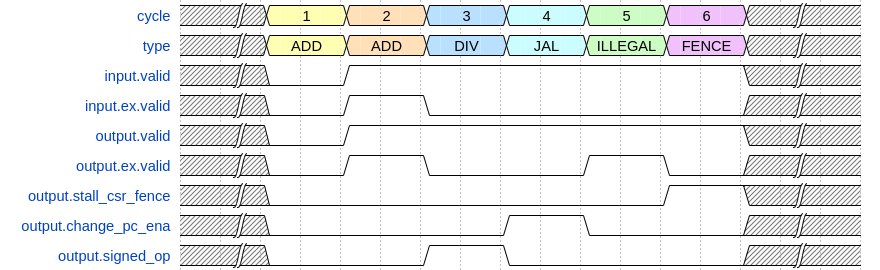
\includegraphics[width=\textwidth]{Figure/full_example.png}
	\caption{Example of expected behavior of the decoder.}
\end{figure}



